\documentclass[journal]{IEEEtran}
\usepackage[T1]{fontenc}
\usepackage{cite}
\usepackage{amsmath,amssymb}
\usepackage{graphicx}
\usepackage{booktabs}
\usepackage{url}
\usepackage{algorithm}
\usepackage{algorithmic}
\usepackage{tikz}
\usetikzlibrary{arrows.meta,positioning}
\graphicspath{{figures/}}
\newcommand{\srp}{SRP-CLAHE-HGPSO}
\newcommand{\clip}{\operatorname{clip}}
\newcommand{\sgn}{\operatorname{sgn}}

\title{Spectral-Ratio-Preserving CLAHE-HGPSO Enhancement of Four-Band Sentinel-2 Images}
\author{Sumaiya~Farhana~Islam, Adnan~Bin~Wahid, Redowan~Billah~Sami,
and Md.~Touhidur~Rahman%
\thanks{\raggedright All authors are with the Institute of Information Technology,
University of Dhaka, Dhaka, Bangladesh.
E-mail: \texttt{bsse1450@iit.du.ac.bd} (S. F. Islam),
\texttt{bsse1442@iit.du.ac.bd} (A. B. Wahid),
\texttt{bsse1409@iit.du.ac.bd} (R. B. Sami), and
\texttt{bsse1432@iit.du.ac.bd} (M. T. Rahman).}}

\begin{document}
\maketitle

\begin{abstract}
Visual enhancement of multispectral satellite imagery can alter band relationships used in quantitative analysis. This paper investigates an image-specific approach that applies a common positive gain to the visible and near-infrared bands of Sentinel-2 imagery. It adapts contrast-limited adaptive histogram equalization (CLAHE) and inherited hybrid grey-wolf and particle-swarm optimization (HGPSO), with feasibility-ranked selection, proxy evaluation, and full-resolution elite checking. Constraints limit changes in vegetation and water indices, mean spectral angle, and clipped band samples. Evaluation uses 200 test chips, nine methods, and auxiliary parameter, repeated-seed, and synthetic experiments. Compared with non-optimized common-gain CLAHE, the proposed method increases mean local RMS contrast by 33.38\%, with a significant paired difference, but decreases input-referenced structural similarity. Mean normalized difference vegetation index (NDVI) error, normalized difference water index (NDWI) error, and spectral angle are $1.95\times10^{-5}$, $5.27\times10^{-5}$, and $0.00530$ degrees, respectively; spectral-error differences from the common-gain control are not significant in the primary chip-level tests. All four constraints hold for 190 of 200 outputs. Mean timed method-stage runtime is 2.805~s, 28.19\% below a larger-budget HGPSO reproduction, but 18.58 times that of common-gain CLAHE. These findings establish a measured contrast--spectral-consistency trade-off, not guaranteed feasibility, preservation of absolute radiometry, or clean-image restoration.
\end{abstract}

\begin{IEEEkeywords}
Multispectral image enhancement, Sentinel-2, contrast-limited adaptive histogram equalization, spectral-ratio preservation, constrained optimization.
\end{IEEEkeywords}

\section{Introduction}
\label{sec:introduction}
\IEEEPARstart{M}{ultispectral} satellite images serve both visual interpretation and quantitative analysis. Improving the appearance of a dark or low-contrast display does not necessarily preserve relationships among the underlying bands. This distinction matters when visible and near-infrared (NIR) values are subsequently used in normalized-difference indices. The normalized difference vegetation index (NDVI) compares red and NIR signals, while the green--NIR normalized difference water index (NDWI) emphasizes a different relationship \cite{rouse1974,mcfeeters1996}. Enhancing visible bands while leaving NIR unchanged can therefore change these indices even when the display becomes more distinctive.

Histogram equalization (HE), contrast-limited adaptive histogram equalization (CLAHE), and adaptive gamma correction with weighting distribution (AGCWD) provide established intensity-enhancement strategies \cite{pizer1987,huang2013}. Image-specific optimization can additionally tune a local transformation. Rentapalli and Khairuzzaman combine CLAHE with hybrid grey-wolf and particle-swarm optimization (HGPSO) for satellite-image enhancement \cite{rentapalli2026}. Such methods motivate a practical question: can optimized display contrast be increased without unnecessary distortion of four-band spectral shape, and at what computational cost?

Applying one positive multiplier to all bands at a pixel preserves their ratios before clipping. Common-channel scaling is an established principle in hue-preserving enhancement \cite{naik2003}; its use here is not presented as a first invention. Nevertheless, multispectral implementation details remain consequential. Gain bounds, numerical safeguards, display-domain offsets, and per-band clipping affect the final behavior. Moreover, optimization adds cost to a property that a non-optimized common-gain method can already provide. A meaningful control must therefore separate the contribution of shared scaling from the contribution of search.

This work examines \srp, a four-band, constraint-aware adaptation of CLAHE-HGPSO. A gain constructed from a transformed display value is applied to blue, green, red, and NIR. A bounded five-parameter search uses a proxy image and checks selected candidates at full resolution. Nine methods are compared on 200 held-out chips from a Sentinel-2 cloud-cover dataset \cite{radiant2022}. The primary control is common-gain CLAHE, which uses the same four-band gain architecture without optimization. RGB-only adapters of classical and optimized methods provide additional context.

The contributions are: 1) an explicitly specified four-band implementation with a qualified ratio-preservation argument; 2) a feasibility-ranked procedure combining an inherited transform and hybrid optimizer with proxy search and full-resolution checking; and 3) an empirical analysis of contrast, spectral errors, failures, cost, and auxiliary sensitivity. The study does not claim a new swarm algorithm, universal image-quality superiority, or improved downstream classification. Sections~\ref{sec:related}--\ref{sec:setup} describe the context, method, and protocol; Sections~\ref{sec:results}--\ref{sec:conclusion} report and interpret the findings.

\section{Related Work}
\label{sec:related}
\subsection{Contrast Enhancement and Image-Specific Search}
Adaptive histogram methods operate locally rather than using only one global mapping, offering an established basis for contrast manipulation \cite{pizer1987}. AGCWD instead derives an adaptive gamma mapping from a weighted intensity distribution \cite{huang2013}. Applying these strategies to a displayed value channel is not equivalent to independently enhancing calibrated multispectral bands.

Particle swarm optimization (PSO) updates positions using velocity, personal history, and population information \cite{poli2007}. The grey wolf optimizer (GWO) uses leader-guided updates \cite{mirjalili2014}. HGPSO combines these ideas with CLAHE and a parameterized transform \cite{rentapalli2026}. This study credits that foundation and independently implements the adopted components. Its five-term visual score, gain adapter, constraints, and evaluation protocol differ from the source study. Published source scores are not measurements of this implementation.

\subsection{Color Consistency and Spectral Shape}
Hue-preserving enhancement highlights common-channel operations and output-gamut handling \cite{naik2003}. Recent work also addresses hue-preserving adjustment through convex-combination coefficient transformations \cite{ueda2025}. Such RGB studies motivate bounded outputs, but do not themselves demonstrate vegetation/water-index preservation in RGB-NIR imagery. Spectral angle measures vector-direction similarity rather than magnitude agreement \cite{kruse1993}. Low angular error can consequently coexist with altered absolute reflectance. Here, index and angle consistency follow primarily from shared gain; constraints check departures associated with clipping and numerical effects.

\subsection{Learned Enhancement and Evaluation Scope}
Learned remote-sensing enhancement is another relevant direction. A spatial--frequency dual-domain network addresses low-light enhancement through amplitude/phase processing and feature fusion \cite{yao2024}. It concerns a different model/data setting from image-specific, training-free parameter search. No learned enhancement model is executed here, so superiority over that class is not established. Similarly, structural similarity (SSIM) must be interpreted relative to its reference \cite{wang2004}. Similarity to the unenhanced input measures input fidelity, not clean-reference restoration. This distinction guides the main evaluation and auxiliary synthetic experiment.

\section{Proposed Method}
\label{sec:method}
\subsection{Input, Mask, and Display Representation}
Let $\mathbf{x}(q)=[B(q),G(q),R(q),N(q)]^\mathsf{T}$ be the stored four-band vector at pixel $q$, and let $\Omega$ denote valid clear pixels. Loading scales source values, excludes invalid/cloud pixels, and verifies band alignment. A visible-band display mapping $D$ uses the original chip's second and 98th percentiles. Every method reuses the same mapping on that chip; enhancement-specific display rescaling is excluded from comparison.

Displayed channels are reordered to RGB and converted to HSV. CLAHE transforms the initial value channel $V_0$ into $o$, using normalized clip limit 0.01, nominal $8\times8$ tiles, and 256 bins. Invalid pixels are filled for local filtering and restored in the returned cube. Gain application and spectral checking operate on the scaled four-band cube, not on displayed RGB. Because $D$ has offsets and clipping, a desired display value need not be reproduced exactly after cube-domain multiplication.

\begin{figure*}[t]
\centering
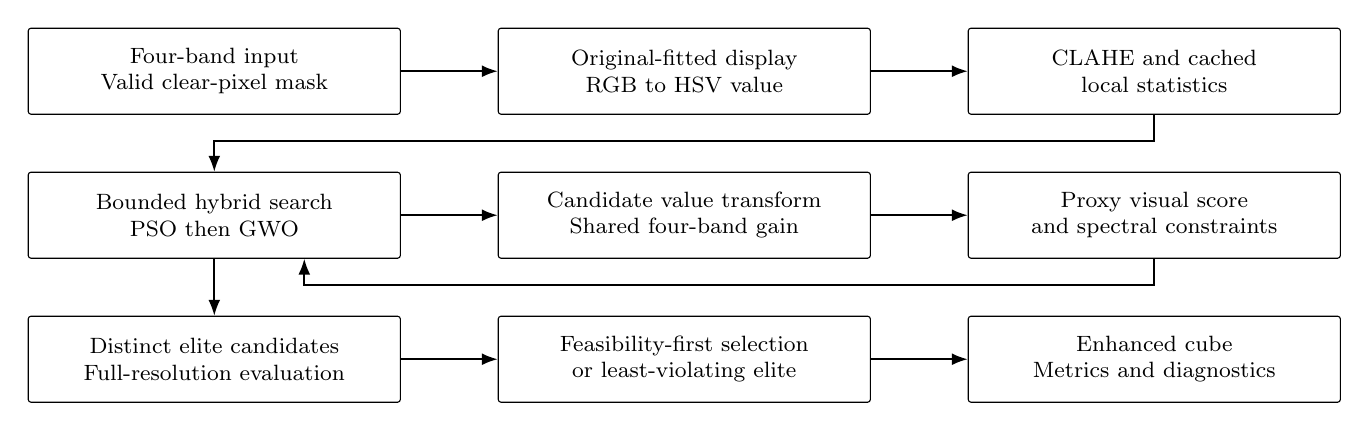
\begin{tikzpicture}[
  box/.style={draw,rectangle,rounded corners=1pt,align=center,
    text width=1.75in,minimum height=0.43in,font=\footnotesize,
    inner sep=4pt,fill=white},
  flow/.style={-{Latex[length=2mm]},semithick}]
\node[box] (cube) at (0,0) {Four-band input\\Valid clear-pixel mask};
\node[box] (display) at (2.35in,0) {Original-fitted display\\RGB to HSV value};
\node[box] (clahe) at (4.70in,0) {CLAHE and cached\\local statistics};
\node[box] (search) at (0,-0.72in) {Bounded hybrid search\\PSO then GWO};
\node[box] (gain) at (2.35in,-0.72in) {Candidate value transform\\Shared four-band gain};
\node[box] (check) at (4.70in,-0.72in) {Proxy visual score\\and spectral constraints};
\node[box] (elite) at (0,-1.44in) {Distinct elite candidates\\Full-resolution evaluation};
\node[box] (select) at (2.35in,-1.44in) {Feasibility-first selection\\or least-violating elite};
\node[box] (output) at (4.70in,-1.44in) {Enhanced cube\\Metrics and diagnostics};
\draw[flow] (cube) -- (display);
\draw[flow] (display) -- (clahe);
\draw[flow] (clahe.south) -- ++(0,-0.13in) -| (search.north);
\draw[flow] (search) -- (gain);
\draw[flow] (gain) -- (check);
\draw[flow] (check.south) -- ++(0,-0.13in) -| ([xshift=0.45in]search.south);
\draw[flow] (search.south) -- (elite.north);
\draw[flow] (elite) -- (select);
\draw[flow] (select) -- (output);
\end{tikzpicture}

\caption{Processing and evaluation pipeline. Display bounds are fitted once to the original chip. Proxy and full-resolution checking use the same gain rule at different resolutions. If no full-resolution elite is feasible, the selector returns a least-violating output rather than guaranteeing feasibility.}
\label{fig:pipeline}
\end{figure*}

\subsection{Parameterized Value Transformation}
The inherited local transform is specified to remove ambiguity in its reproduction \cite{rentapalli2026}. For local uniform-window mean $m$, local second moment $s_2$, global valid-pixel mean $\mu$, and parameters $\boldsymbol{\theta}=(a,b,c,k,p)$, define
\begin{align}
\sigma_c&=\sqrt{\max\{s_2+(c^2-2c)m^2,10^{-10}\}},\\
E_{\boldsymbol{\theta}}&=
\frac{k\mu^{\eta}}{\max\{\sigma_c^{\ell}+b,10^{-8}\}}
\sgn(o-cm)(|o-cm|+10^{-12})^{p}\nonumber\\
&\quad+\max\{m,0\}^{a}.
\end{align}
The implementation uses $\eta=\ell=1$ and a $7\times7$ reflected-boundary window. With valid-pixel percentiles $Q_1,Q_{99}$ of $E_{\boldsymbol{\theta}}$, robust rescaling gives
\begin{equation}
V_{\boldsymbol{\theta}}=\clip\left(
\frac{E_{\boldsymbol{\theta}}-Q_1}{Q_{99}-Q_1},0,1\right).
\label{eq:transform}
\end{equation}
A nonpositive percentile range is replaced by $10^{-6}$; small-sample/nonfinite safeguards are specified in code. The $c$-dependent variance, signed fractional power, boundary rule, fixed exponents, and rescaling are disclosed reproduction assumptions rather than exact source-code equivalence. Bounds are $a\in[0.1,1.5]$, $b\in[0.1,0.5]$, $c\in[0.1,1]$, $k\in[0.5,1.5]$, and $p\in[0.1,2]$.

\subsection{Shared Gain and Qualified Preservation}
The positive gain and output are
\begin{align}
r(q)&=\clip\left(\frac{V_{\boldsymbol{\theta}}(q)+\epsilon}
{V_0(q)+\epsilon},r_{\min},r_{\max}\right),\label{eq:gain}\\
y_b(q)&=\clip\big(r(q)x_b(q),0,1\big),\quad b\in\{B,G,R,N\}.
\label{eq:output}
\end{align}
Selected settings are $\epsilon=10^{-4}$ and $[r_{\min},r_{\max}]=[0.5,2]$. Optional mask-normalized Gaussian gain smoothing is disabled in the main experiment ($\sigma=0$). Invalid pixels use gain one and are restored to their inputs.

Before clipping, one positive scalar preserves ratios and vector direction for non-degenerate vectors:
\begin{equation}
\frac{r x_i}{r x_j}=\frac{x_i}{x_j},\qquad
\angle(\mathbf{x},r\mathbf{x})=0.
\end{equation}
It follows that ideal NDVI and McFeeters green--NIR NDWI,
\begin{equation}
I_v=\frac{N-R}{N+R},\qquad I_w=\frac{G-N}{G+N},
\label{eq:indices}
\end{equation}
are invariant for nonzero denominators and unclipped positive gain \cite{rouse1974,mcfeeters1996}. Absolute radiometry is not invariant: $r\mathbf{x}$ generally has a different magnitude.

Measured indices add $\delta=10^{-8}$ to their denominators. A generic difference index after scaling becomes $(u-v)/(u+v+\delta/r)$ instead of $(u-v)/(u+v+\delta)$. Numerical differences can therefore persist without clipping, particularly for dark pixels. Spectral-angle calculations also use numerical safeguards. Per-band clipping in (\ref{eq:output}) can break the common-scalar relationship and cause larger errors. Preservation is thus qualified, not unconditional.

\subsection{Visual Score and Feasibility}
The visual terms are display-luma entropy $H$, local RMS contrast $C$, Canny edge density $E$, Laplacian variance $L$, and input SSIM $S$. Their weights are
\begin{equation}
\mathbf{w}=(0.25,0.25,0.20,0.15,0.15).
\end{equation}
Within each population, the first four terms are normalized using the 10th/90th percentiles and clipped to $[0,1]$. Flat ranges receive 0.5 and nonfinite values zero; SSIM is clipped to $[0,1]$. The population-relative score is
\begin{equation}
Q_{\mathrm{vis}}=w_H\widehat H+w_C\widehat C+w_E\widehat E
+w_L\widehat L+w_SS.
\end{equation}
It ranks the current population, not cross-generation absolute quality.

A separate stable utility $U$ supports historical bookkeeping and stopping. Entropy is divided by eight. For contrast and edge density, a candidate/input ratio $z$ maps to $\clip((z-0.5)/(2.5-0.5),0,1)$; Laplacian variance uses cap three rather than 2.5. Original denominators are floored at $10^{-8}$, SSIM is clipped to $[0,1]$, and the same weights apply. Neither $U$ nor $Q_{\mathrm{vis}}$ is independently validated as a perceptual-quality index.

The constrained errors are
\begin{align}
e_v&=\frac{1}{|\Omega|}\sum_{q\in\Omega}|I_v(\mathbf y(q))-I_v(\mathbf x(q))|,\\
e_w&=\frac{1}{|\Omega|}\sum_{q\in\Omega}|I_w(\mathbf y(q))-I_w(\mathbf x(q))|,\\
e_a&=\frac{1}{|\Omega|}\sum_{q\in\Omega}\angle(\mathbf x(q),\mathbf y(q)),\\
e_c&=\frac{\sum_{q\in\Omega}\sum_b\mathbb{1}\{r(q)x_b(q)\notin[0,1]\}}
{4|\Omega|}.
\end{align}
Angles are in degrees. Clipping counts band samples, not unique clipped pixels. Thresholds for $(e_v,e_w,e_a,e_c)$ are $(0.005,0.005,0.5,0.005)$; normalized violation is
\begin{equation}
\nu=\sum_{j\in\{v,w,a,c\}}\max\{e_j/\tau_j-1,0\}.
\end{equation}
Feasible candidates rank above infeasible candidates. Feasible population ranking uses $Q_{\mathrm{vis}}$ then $U$; infeasible ranking uses smaller $\nu$ then $U$. Historical comparison uses feasibility and stable utility, or smaller violation if infeasible.

\subsection{Hybrid Search and Full-Resolution Checking}
The inherited hybrid evaluates a population, updates historical bests, and applies a PSO step followed by GWO refinement \cite{rentapalli2026,poli2007,mirjalili2014}. PSO inertia is 0.729 and both acceleration constants are 1.49445. Three current leaders guide GWO; its coefficient decreases from two to zero across the configured horizon. Positions are clipped to bounds and initial velocities span $\pm0.1$ of parameter ranges. Intermediate PSO positions are not evaluated as an additional population.

More explicitly, for candidate position $\mathbf t_i$, velocity $\mathbf v_i$, personal best $\mathbf b_i$, and historical global best $\mathbf g$, the PSO intermediate is
\begin{align}
\mathbf v_i'&=\omega\mathbf v_i+c_1\mathbf u_1\odot(\mathbf b_i-\mathbf t_i)
+c_2\mathbf u_2\odot(\mathbf g-\mathbf t_i),\\
\mathbf z_i&=\clip_{\mathcal B}(\mathbf t_i+\mathbf v_i'),
\end{align}
where $\mathcal B$ is the parameter box and random vectors are uniform in $[0,1]$. Current leaders $\mathbf l_j$ then yield
\begin{equation}
\mathbf t_i'=\clip_{\mathcal B}\left(\frac{1}{3}\sum_{j=1}^{3}
\left[\mathbf l_j-\mathbf A_j\odot|\mathbf C_j\odot\mathbf l_j-\mathbf z_i|\right]\right),
\end{equation}
with independent $\mathbf A_j=2a_t\mathbf u_j-a_t$, $\mathbf C_j=2\widetilde{\mathbf u}_j$, and $a_t=2-2t/\max(T-1,1)$ for horizon $T$. Products and absolute values are elementwise.

Proposed search uses population eight, at most 12 generations, and a $256\times256$ proxy. Band resizing uses area interpolation; mask resizing uses nearest neighbor. Full-resolution original display bounds are reused. Stopping uses patience eight and tolerance $10^{-4}$ on stable progress, or negative violation for an infeasible historical best, subject to the minimum-generation condition.

Up to four distinct candidates from the historical best and ranked final population are checked on the $512\times512$ chip. Final selection prefers feasibility then $U$. With no feasible elite, it returns the least-violating one; there is no identity fallback or clipping-safe projection. Algorithm~\ref{alg:search} and Fig.~\ref{fig:pipeline} separate search preference from an output guarantee.

\begin{algorithm}[t]
\caption{Shared-gain enhancement with elite checking}
\label{alg:search}
\begin{algorithmic}[1]
\REQUIRE Four-band cube, valid mask, frozen settings
\STATE Fit original display bounds; build proxy/full contexts.
\STATE Initialize bounded parameters and velocities.
\FOR{each generation until the limit or early stopping}
\STATE Evaluate transform, gain, visual terms, constraints.
\STATE Rank by feasibility; update leaders and bests.
\STATE Record stable progress; check stagnation.
\STATE Apply PSO then GWO updates within bounds.
\ENDFOR
\STATE Evaluate distinct elites at full resolution.
\STATE Choose highest-utility feasible elite, if available;
\STATE otherwise choose the least-violating elite.
\STATE Restore invalid pixels; return output and diagnostics.
\end{algorithmic}
\end{algorithm}

\section{Experimental Setup}
\label{sec:setup}
\subsection{Dataset, Selection, and Calibration}
The source is the Radiant Earth Sentinel-2 Cloud Cover Segmentation Dataset, version one, distributed under CC BY 4.0 \cite{radiant2022}. The study uses 240 selected L2A chips: 40 available validation and 200 test chips. Each is $512\times512$ with B02, B03, B04, and B08 at 10-m sampling. Expert cloud masks exclude clouds; this is neither cloud removal nor an enhancement benchmark with pristine targets.

Loading requires matching shapes, coordinate reference systems, and transforms. Valid pixels are finite, non-nodata, positive in all four bands, and outside cloud labels 1/255. Automatic scaling divides by 10,000 when the valid-sample 99.5th percentile exceeds two, otherwise by one. The outputs are described as reflectance-like scaled values, not independently revalidated radiometric products. Configured minimum validity is 0.70; selected test minimum and mean are 0.9503 and 0.9894, respectively, indicating a mostly clear subset.

Representative subset selection sorts by cloud fraction, valid fraction, and chip identifier, then takes spaced indices. It is deterministic, not seeded random sampling. Validation/test have 13/50 location/acquisition-time groups with no overlapping group or location labels. This metadata separation does not prove disjoint geographic footprints. Test acquisitions span March 2018 to September 2020.

Only six validation chips participate in calibration. Three sequential one-factor stages consider local windows $\{7,15,31\}$, smoothing $\{0,1,2\}$, and upper gain bounds $\{1.5,2,2.5\}$, with 18 candidate-chip evaluations per stage and 54 total. Calibration uses population eight, at most 12 generations, proxy size 256, and three elites. Selection prioritizes feasible rate, median stable utility, then lower median violation/time. This is not a full joint grid search. Window seven, zero smoothing, and gain range $[0.5,2]$ are frozen before main testing. Table~\ref{tab:settings} gives executed settings rather than larger unused presets.

\begin{table}[t]
\centering\footnotesize
\caption{Dataset and executed settings. P/G: population/maximum generations. Actual evaluation counts vary with stopping.}
\label{tab:settings}
\begin{tabular}{@{}lp{0.57\columnwidth}@{}}\toprule
Item & Setting \\\midrule
Validation/test & 40 available / 200 test chips \\
Calibration & 6 chips; 54 candidate-chip runs \\
Main spatial sizes & $512\times512$ full; $256\times256$ proxy \\
Display / transform & 2nd/98th / 1st/99th percentiles \\
CLAHE & Clip 0.01; $8\times8$ tiles; 256 bins \\
Shared gain & $[0.5,2]$; $\epsilon=10^{-4}$; smoothing 0 \\
SRP search & P/G $8/12$; four full-resolution elites \\
PSO/GWO/HGPSO & P/G $10/20$; one full candidate \\
Stopping & Patience 8; tolerance $10^{-4}$ \\
Spectral limits & NDVI/NDWI MAE 0.005; SAM $0.5^\circ$ \\
Clipping limit & 0.005 of valid band samples \\
Auxiliary runs & Ablation: 8 chips/20 variants; seeds: 8 chips/3 seeds; synthetic: 12 chips \\
\bottomrule\end{tabular}
\end{table}

\subsection{Baselines, Budgets, and Environment}
The methods are Original, HE, CLAHE, AGCWD, common-gain CLAHE, PSO, GWO, HGPSO, and \srp. Original applies no enhancement. Classical baselines are independently implemented on HSV value; AGCWD uses weighting exponent 0.5. HE/CLAHE/AGCWD apply a visible-band gain in $[0.05,20]$ to B/G/R with unchanged NIR. PSO/GWO/HGPSO use the inherited transform and common visual score with this RGB-only adapter, without spectral constraints. Their population is ten, maximum generations 20, proxy size 256, and full-resolution candidate count one. HGPSO is an independent reproduction under Section~\ref{sec:method}'s assumptions, not the source authors' software or exact experimental results.

Common-gain CLAHE directly uses CLAHE without parameter search, applies gain to all four bands, and shares proposed gain bounds/smoothing. It is the closest architectural control. Proposed and RGB-only methods differ in adapter, gain bounds, feasibility treatment, elite count, and budget. Their comparison does not isolate an optimizer-only causal effect or matched-budget speedup.

The base seed is 20260817; method/chip/experiment tags deterministically derive run-specific seeds. The saved environment records Windows 11, Python 3.12.4, 16 logical/ten physical CPUs, and 15.773~GB RAM; the exact CPU product name is absent. Recorded versions include NumPy 2.5.2, SciPy 1.18.0, pandas 2.3.3, OpenCV 4.14.0.94, scikit-image 0.26.0, Matplotlib 3.11.1, and rasterio 1.5.1. Execution is sequential without claimed GPU acceleration. Main results come solely from the completed standard-run archive.

\subsection{Metrics, Timing, and Statistical Procedure}
Display luma is $0.2126R_d+0.7152G_d+0.0722B_d$, without sRGB gamma linearization. Entropy uses 256 bins after 8-bit quantization. Local RMS contrast averages local standard deviations from a reflected-boundary $7\times7$ uniform filter. Edge density is the valid-pixel fraction detected by Canny at thresholds 50/150; sharpness is Laplacian variance on 8-bit luma. These descriptors do not independently prove perceptual improvement or recovered scene information.

Input SSIM uses a full scikit-image similarity map, data range one, default uniform $7\times7$ window, and sample covariance, then valid-mask averaging \cite{wang2004,skimageDocs}. This differs from canonical Gaussian-window SSIM settings. Filtering and SSIM neighborhoods may include filled invalid pixels despite masked averaging. Spectral metrics reference the input cube. SAM uses float64 arithmetic, numerical denominator safeguards, and near-one cosine snapping. Main tables give arithmetic chip means and sample standard deviations.

Runtime is the timed method stage, excluding scene I/O and context/display preparation but including candidate metrics and elite checking. Optimized context construction includes CLAHE caches outside the timer; simple methods execute enhancement inside it. These boundaries exclude end-to-end cost. A descriptive pixel-equivalent workload is $n_p(P/F)+n_f$, where $n_p,n_f$ count proxy/full evaluations and $P,F$ are their pixel counts. It is not a validated complexity or hardware-normalized cost model.

Paired two-sided Wilcoxon signed-rank tests compare the proposed method with seven enhancement controls; Original is excluded. Holm correction is applied separately to each metric's seven-comparison family \cite{holm1979}. Positive oriented rank-biserial effects favor SRP, reversing signs for lower-is-better metrics. Ties use exact equality and zero differences are omitted. The audit agrees with archived significance decisions; correcting a near-tie effect helper changes effects by at most 0.0192, not conclusions. SciPy's automatic test method and recorded version determine tie/zero treatment \cite{scipyDocs}.

Chip dependence motivates post hoc sensitivity: average each method within location/acquisition-time groups, then compare 50 paired group means using the same per-metric correction. Groups approximate acquisition context, not verified independent geography. Structured dependence remains a limitation \cite{roberts2017}; non-significance does not establish equivalence.

The signed-rank location-shift interpretation also depends on the distribution of paired differences, including its symmetry. The very small adjusted probabilities are reported under this test convention, not as proof of independent geographic replication.

\section{Results}
\label{sec:results}
\begin{table*}[t]
\centering\footnotesize
\caption{Test-set results (200 chips): mean $\pm$ sample standard deviation. Spectral errors are relative to the input. Clipping counts band samples; times are measured method stages, not end-to-end processing. RGB-only adapters leave NIR unchanged; common-gain CLAHE and SRP apply gain to all four bands.}
\label{tab:main}
\textit{(a) Display descriptors and measured cost}\par\smallskip
\begin{tabular*}{\textwidth}{@{\extracolsep{\fill}}lrrrr@{}}
\toprule
Method & Entropy (bits) & Local RMS contrast & Input SSIM & Time (s) \\
\midrule
Original & $7.445 \pm 0.470$ & $0.084 \pm 0.042$ & $1.000 \pm 0.000$ & $0.082 \pm 0.018$ \\
HE & $6.846 \pm 0.818$ & $0.150 \pm 0.072$ & $0.499 \pm 0.215$ & $0.127 \pm 0.028$ \\
CLAHE & $7.226 \pm 0.594$ & $0.171 \pm 0.078$ & $0.536 \pm 0.137$ & $0.152 \pm 0.035$ \\
AGCWD & $6.725 \pm 1.343$ & $0.100 \pm 0.047$ & $0.527 \pm 0.202$ & $0.130 \pm 0.030$ \\
Common-gain CLAHE & $7.256 \pm 0.601$ & $0.167 \pm 0.080$ & $0.548 \pm 0.142$ & $0.151 \pm 0.037$ \\
PSO & $7.316 \pm 0.481$ & $0.212 \pm 0.086$ & $0.439 \pm 0.123$ & $5.032 \pm 1.564$ \\
GWO & $7.272 \pm 0.506$ & $0.221 \pm 0.082$ & $0.418 \pm 0.130$ & $3.615 \pm 1.267$ \\
HGPSO & $7.312 \pm 0.514$ & $0.217 \pm 0.082$ & $0.426 \pm 0.129$ & $3.906 \pm 1.481$ \\
SRP-CLAHE-HGPSO & $7.226 \pm 0.600$ & $0.223 \pm 0.094$ & $0.429 \pm 0.126$ & $2.805 \pm 0.779$ \\
\bottomrule\end{tabular*}
\medskip\textit{(b) Spectral consistency and clipping}\par\smallskip
\begin{tabular*}{\textwidth}{@{\extracolsep{\fill}}lrrrr@{}}
\toprule
Method & NDVI MAE ($10^{-3}$) & NDWI MAE ($10^{-3}$) & SAM (degrees) & Clipping (\%) \\
\midrule
Original & $0.0000 \pm 0.0000$ & $0.0000 \pm 0.0000$ & $0.0000 \pm 0.0000$ & $0.0000 \pm 0.0000$ \\
HE & $164.1272 \pm 121.0751$ & $164.5152 \pm 125.1688$ & $8.8581 \pm 6.6294$ & $0.2977 \pm 1.9562$ \\
CLAHE & $128.4385 \pm 47.8654$ & $130.1417 \pm 49.3795$ & $7.0572 \pm 3.0391$ & $0.4953 \pm 2.2562$ \\
AGCWD & $126.5877 \pm 48.0924$ & $126.5178 \pm 47.9271$ & $6.8120 \pm 2.9435$ & $0.7180 \pm 5.0739$ \\
Common-gain CLAHE & $0.0414 \pm 0.2979$ & $0.0962 \pm 0.7160$ & $0.0115 \pm 0.1002$ & $0.2885 \pm 2.1919$ \\
PSO & $148.6431 \pm 87.0739$ & $150.5154 \pm 92.0422$ & $8.1494 \pm 5.1467$ & $0.3333 \pm 1.5493$ \\
GWO & $155.6273 \pm 86.2391$ & $157.4263 \pm 89.2145$ & $8.4825 \pm 5.0318$ & $0.3548 \pm 1.4805$ \\
HGPSO & $150.4994 \pm 74.9857$ & $152.3387 \pm 76.7472$ & $8.2245 \pm 4.3211$ & $0.3316 \pm 1.5016$ \\
SRP-CLAHE-HGPSO & $0.0195 \pm 0.0994$ & $0.0527 \pm 0.3286$ & $0.0053 \pm 0.0374$ & $0.1391 \pm 0.8338$ \\
\bottomrule\end{tabular*}
\end{table*}

\subsection{Visual Contrast and Spectral Consistency}
Table~\ref{tab:main} summarizes all 1,800 main observations. Mean local RMS contrast is 0.22306 for SRP, versus 0.16724 for common-gain CLAHE, 0.17130 for CLAHE, and 0.08391 for Original. Ratios of arithmetic means give increases of 33.38\%, 30.22\%, and 165.85\%, respectively. The closest-control contrast comparison has adjusted $p=1.108\times10^{-30}$ and effect $r=0.952$ (Table~\ref{tab:stats}). Search adds a clear contrast difference over shared-gain CLAHE in these runs.

This benefit has a fidelity trade-off. Mean input SSIM falls from 0.54840 for common-gain CLAHE to 0.42917 for SRP, with adjusted $p=9.498\times10^{-27}$ and $r=-0.888$. Proposed entropy, 7.22639 bits, is below Original's 7.44479 and close to CLAHE's 7.22594. Entropy differences from common-gain CLAHE and HGPSO are not significant after primary correction. Higher local contrast is not synonymous with higher entropy or input similarity.

Mean proposed NDVI MAE, NDWI MAE, and SAM are $1.948\times10^{-5}$, $5.267\times10^{-5}$, and $0.005299^\circ$. Common-gain CLAHE likewise has small errors: $4.142\times10^{-5}$, $9.619\times10^{-5}$, and $0.011549^\circ$. Primary adjusted $p$ values are 0.7427, 0.7189, and 0.2705; significant spectral improvement from search is not established. Many angular differences are exactly zero under the numerical metric convention.

RGB-only HGPSO instead has mean NDVI MAE 0.15050, NDWI MAE 0.15234, and SAM $8.22454^\circ$. Each corresponding comparison has adjusted $p=1.005\times10^{-33}$ and effect one. This is consistent with changing visible values while leaving NIR unchanged, not proof that search discovers a new preservation principle. Proposed mean contrast exceeds HGPSO by 2.89\%, but adjusted paired $p$ is one and the paired median difference is slightly negative. Contrast superiority over HGPSO is not established.

\begin{figure*}[t]
\centering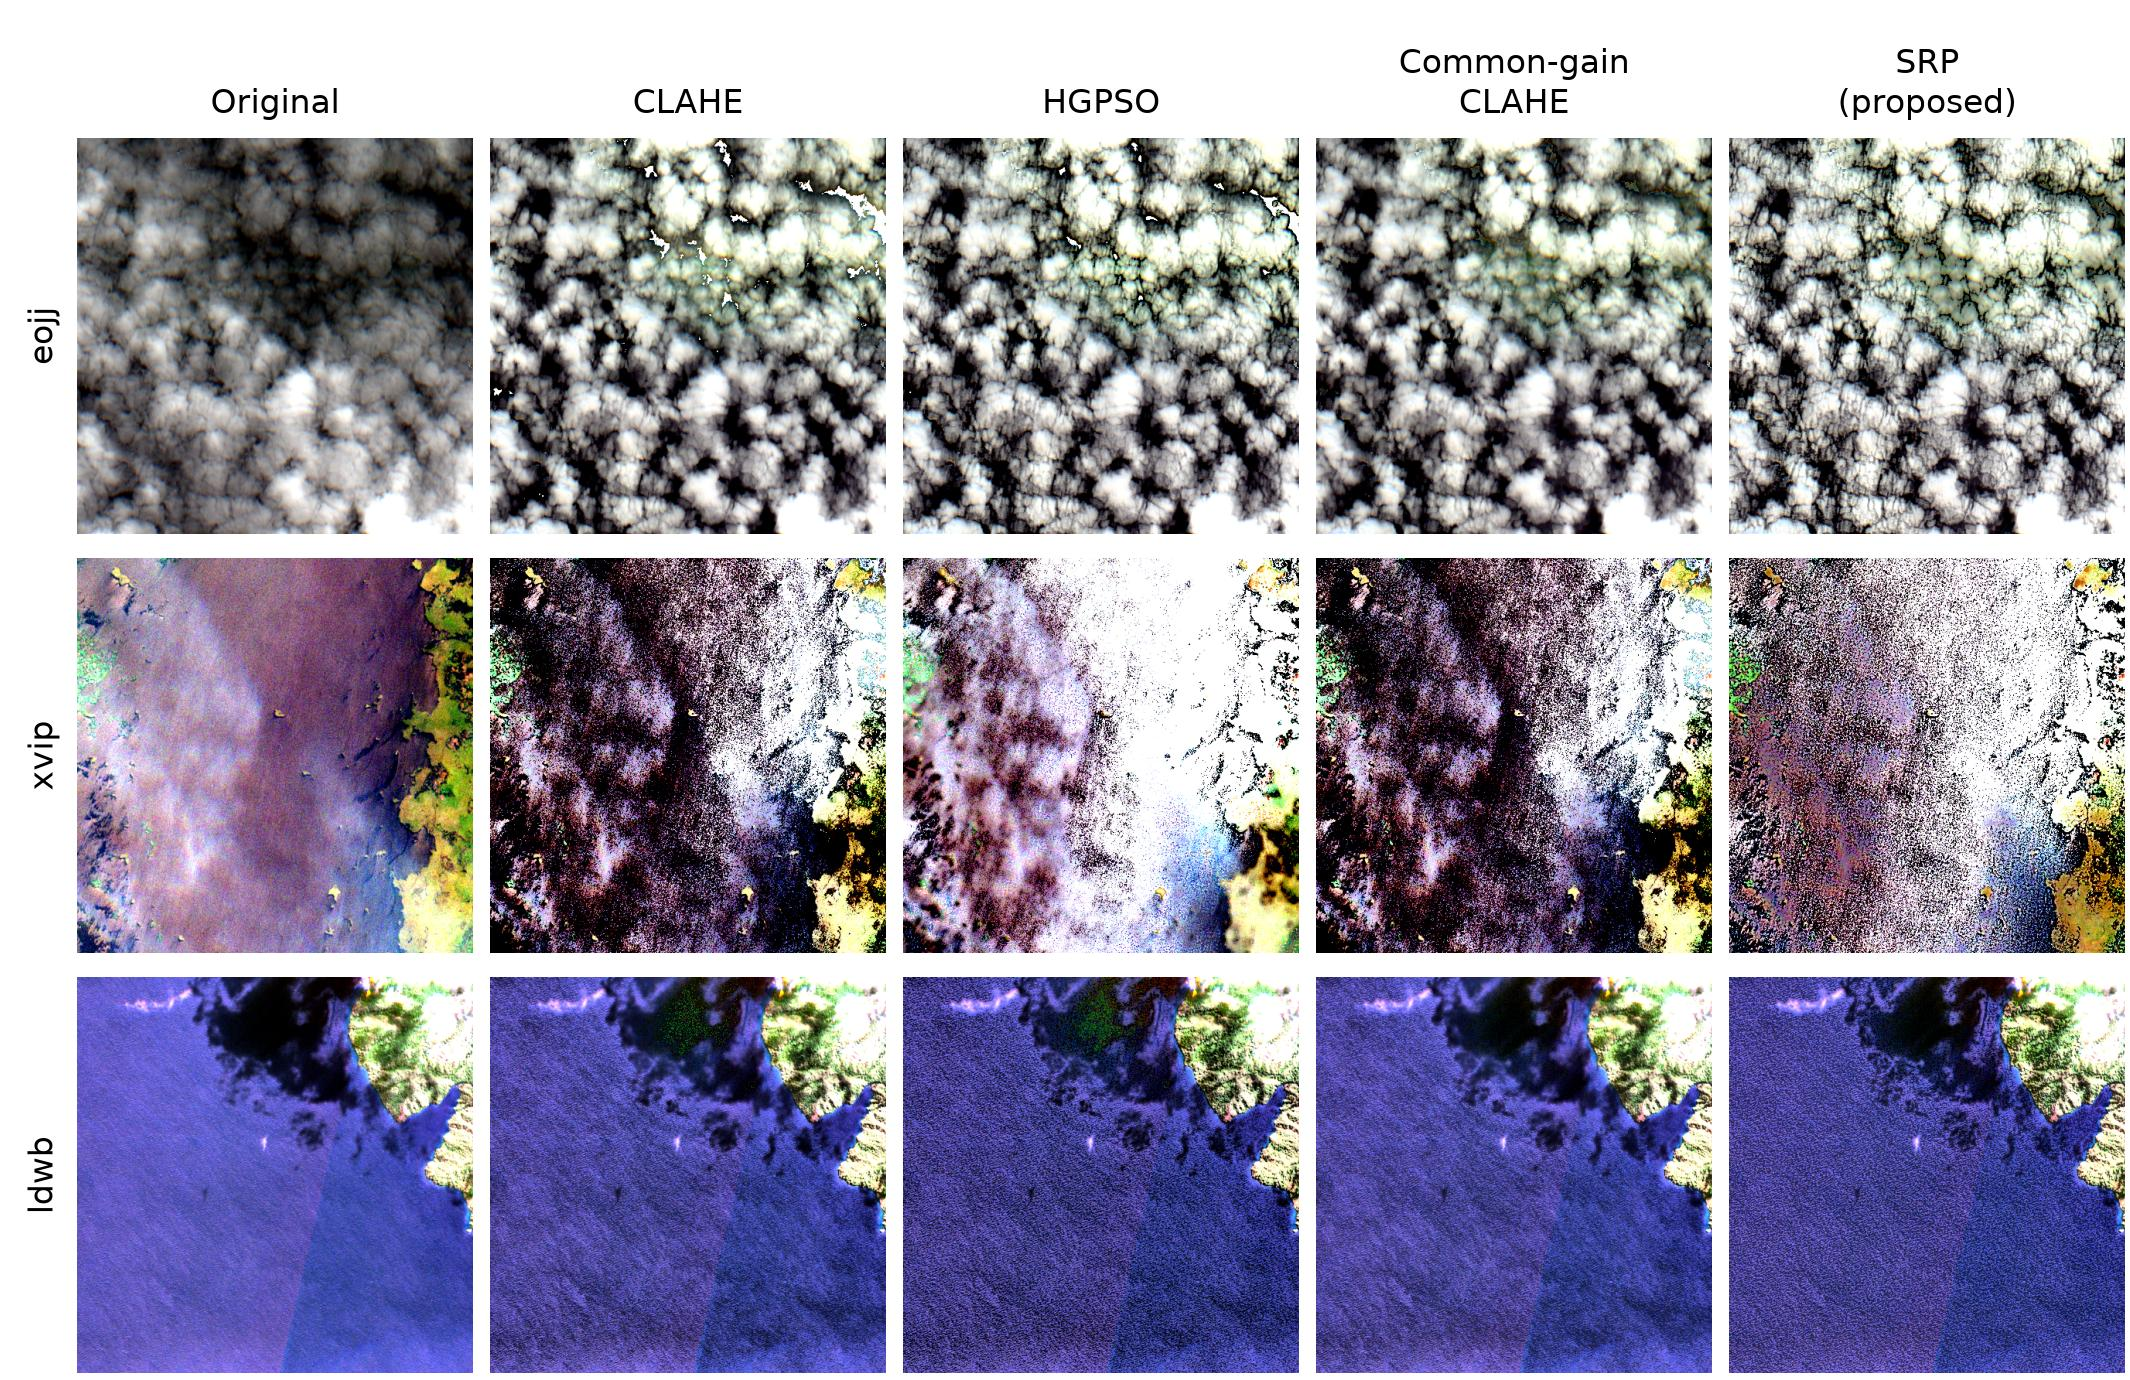
\includegraphics[width=\textwidth]{qualitative.jpg}
\caption{Saved RGB displays with identical original-fitted bounds per chip. Rows are selected from eight archived qualitative chips by lowest original contrast, upper-median original contrast, and greatest proposed clipping; ties use chip ID. These illustrate appearance changes, not subjective preference or the worst case among all 200 chips.}
\label{fig:qualitative}
\end{figure*}

\begin{figure*}[t]
\centering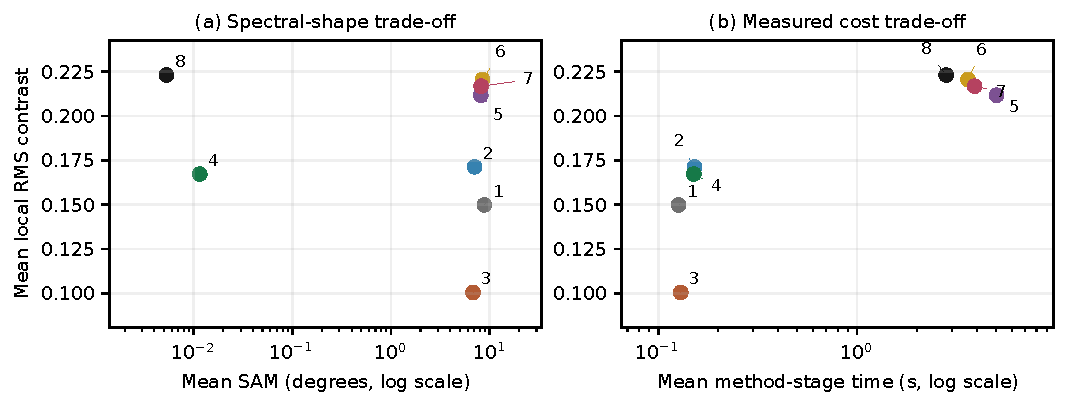
\includegraphics[width=\textwidth]{tradeoffs.pdf}
\caption{Test-set means: (a) contrast versus spectral angle and (b) contrast versus measured stage time. Horizontal axes are logarithmic. Keys: 1 HE, 2 CLAHE, 3 AGCWD, 4 common-gain CLAHE, 5 PSO, 6 GWO, 7 HGPSO, 8 SRP. Original is omitted because its angle is zero. Means do not establish a universal Pareto guarantee.}
\label{fig:tradeoff}
\end{figure*}

\subsection{Statistical Sensitivity and Constraint Failures}
\begin{table}[t]\centering\footnotesize
\caption{Selected proposed-versus-control tests on 200 chips. CG: common-gain CLAHE; HG: HGPSO. Holm correction covers seven controls separately per metric. Positive oriented rank-biserial effect $r$ favors SRP.}
\label{tab:stats}\begin{tabular}{@{}llrr@{}}\toprule
Control & Metric & Adjusted $p$ & $r$ \\\midrule
CG & Contrast & $1.11\times10^{-30}$ & $+0.952$ \\
CG & Input SSIM & $9.50\times10^{-27}$ & $-0.888$ \\
CG & NDVI MAE & $0.7427$ & $-0.027$ \\
CG & NDWI MAE & $0.7189$ & $-0.029$ \\
CG & SAM & $0.2705$ & $+0.165$ \\
CG & Time & $1.01\times10^{-33}$ & $-1.000$ \\
HG & Contrast & $1.0000$ & $+0.054$ \\
HG & NDVI MAE & $1.01\times10^{-33}$ & $+1.000$ \\
HG & NDWI MAE & $1.01\times10^{-33}$ & $+1.000$ \\
HG & SAM & $1.01\times10^{-33}$ & $+1.000$ \\
HG & Time & $9.88\times10^{-27}$ & $+0.878$ \\
\bottomrule\end{tabular}\end{table}

The archived Friedman contrast omnibus statistic is 805.202 with $p=1.400\times10^{-169}$ across eight enhancement methods and 200 blocks. This indicates differences among methods, not superiority over every control. Selected paired tests supply the more relevant contrasts.

With group-level aggregation, contrast versus common-gain CLAHE remains significant ($p=2.132\times10^{-14}$) and contrast versus HGPSO remains non-significant ($p=0.4595$). HGPSO spectral-error/runtime comparisons remain significant. Other findings change: proposed entropy is lower than HGPSO ($p=0.0286$), while SAM and clipping versus common-gain CLAHE become significant ($p=0.00582$ and $0.00566$) despite very small/zero-centered differences. These changes caution against automatic independence assumptions and selective reporting.

Full-resolution checks identify 190/200 joint-feasible outputs (95\%). All 200 meet NDVI, NDWI, and mean-SAM limits; ten exceed the clipping limit. Maximum proposed NDVI MAE, NDWI MAE, and mean SAM are approximately 0.000897, 0.004046, and $0.48981^\circ$. Maximum clipping is 0.100465, or 10.0465\% of valid band samples. Thus, mean clipping of 0.001391 hides a substantive worst-case failure. Proxy preference and elite checking are not guarantees.

Fig.~\ref{fig:qualitative} uses a documented rule on saved chips, not selection solely favoring SRP. Outputs alter texture, brightness, and contrast, but no subjective study certifies preference. Fig.~\ref{fig:tradeoff} separates spectral shape from cost: common-gain CLAHE supplies a much cheaper low-error operating point.

\subsection{Measured Cost and Convergence}
Mean time is $2.805\pm0.779$~s for SRP versus $3.906\pm1.481$~s for HGPSO, a 28.19\% reduction in the ratio of means, with adjusted $p=9.879\times10^{-27}$. Budgets and elite counts differ. Proposed search averages 92.68 proxy plus four full evaluations; HGPSO averages 146 plus one. Pixel-equivalent workloads are 27.17 and 37.5. The time difference describes the executed configurations, not isolated algorithmic efficiency.

Common-gain CLAHE averages 0.15095~s, making SRP 18.58 times slower on this stage. It is a serious alternative when low spectral error and minimal cost matter. Whether additional contrast justifies search depends on the workflow; real-time deployment and end-to-end latency are not established.

\begin{figure}[t]
\centering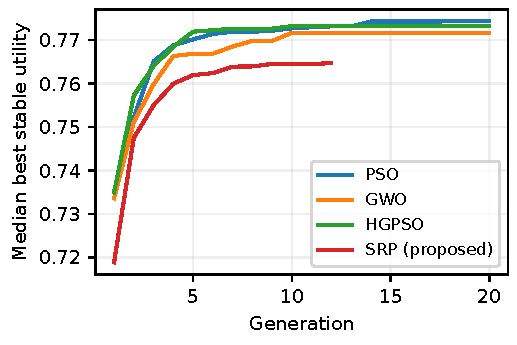
\includegraphics[width=\columnwidth]{convergence.pdf}
\caption{Median best stable utility over 200 main-test chips per optimizer. Early-stopped histories carry their last values forward within the observed horizon: 12 generations for SRP, 20 for controls. Generations do not represent equal work/time, and utility is not an independent perceptual-quality score.}
\label{fig:convergence}
\end{figure}

Fig.~\ref{fig:convergence} includes only main-test histories, excluding auxiliary namespaces. Its curves describe progress in stable bookkeeping utility. The lower proposed curve is not suppressed or interpreted as universal quality inferiority: candidate architecture and feasible search space differ. Conversely, a shorter horizon does not prove convergence to an equally good solution at lower cost.

\subsection{Parameter Sensitivity and Repeated Seeds}
\begin{table}[t]\centering\footnotesize
\caption{Selected sensitivity runs: means over eight chips. Different seed tags across variants confound setting and search randomness; these are descriptive comparisons.}
\label{tab:ablation}
\begin{tabular}{@{}lrrr@{}}\toprule
Setting & Contrast & NDVI MAE & Time (s) \\\midrule
Without constraints & 0.2370 & $8.07\times10^{-8}$ & 2.182 \\
Smoothing $\sigma=0$ & 0.2584 & $8.21\times10^{-8}$ & 2.166 \\
Smoothing $\sigma=1$ & 0.1984 & $4.02\times10^{-8}$ & 2.601 \\
Smoothing $\sigma=2$ & 0.1354 & $3.40\times10^{-8}$ & 2.560 \\
Gain $[0.4,2.5]$ & 0.2171 & $8.39\times10^{-6}$ & 2.387 \\
Gain $[0.5,2.0]$ & 0.2271 & $7.72\times10^{-8}$ & 2.328 \\
Gain $[0.7,1.5]$ & 0.2267 & $3.35\times10^{-8}$ & 2.368 \\
Proxy $128\times128$ & 0.2550 & $7.88\times10^{-8}$ & 0.904 \\
Proxy $256\times256$ & 0.2401 & $8.10\times10^{-8}$ & 2.215 \\
Proxy $512\times512$ & 0.2127 & $7.30\times10^{-8}$ & 11.361 \\
\bottomrule\end{tabular}\end{table}

Twenty variants run on eight chips. Table~\ref{tab:ablation} selects smoothing, gain bounds, proxy size, and constraint removal; other variants examine search budget, reduced parameter search, and weights. Different seed tags confound setting and search randomness, so these are descriptive rather than seed-matched causal ablations.

Mean contrast decreases from 0.2584 at smoothing $\sigma=0$ to 0.1984 at one and 0.1354 at two. Wider bounds $[0.4,2.5]$ admit more index error, whereas $[0.7,1.5]$ achieves similar contrast to $[0.5,2]$ and zero mean clipping on this subset. Selected bounds are not uniquely optimal. Removing constraints still gives tiny errors on these eight chips, supporting shared gain as the main preservation mechanism rather than proving constraints necessary.

Proxies 128, 256, and 512 give times 0.904, 2.215, and 11.361~s. Smaller proxies reduce cost, but contrast is not monotonic and equal-quality equivalence is unproved. Larger population/generation settings do not improve every metric monotonically and differ from the main $8/12$ setting. Full-test main means are therefore not matched eight-chip controls. Weight variants define different utilities, requiring comparison of raw descriptors instead of differently weighted utility scores.

Repeated-seed analysis uses eight chips, three seeds, and two methods. Variation is computed within each chip, then summarized across chips; pooling 24 outputs would mix scene and seed variation. Median within-chip utility standard deviation is 0.00852 for SRP and 0.00600 for HGPSO. SRP is not uniformly more stable in visual utility. Relative variability of near-zero spectral errors is difficult to interpret, and three seeds give limited stochastic-tail evidence.

\subsection{Auxiliary Synthetic Reference Evaluation}
\begin{table}[t]\centering\footnotesize
\caption{Auxiliary synthetic results (12 chips): clean-reference scores, mean $\pm$ SD. Original denotes the degraded input with no enhancement.}
\label{tab:synthetic}\begin{tabular}{@{}lrr@{}}\toprule
Method & PSNR (dB) & SSIM \\\midrule
Original & $12.142 \pm 4.750$ & $0.518 \pm 0.223$ \\
CLAHE & $9.819 \pm 2.979$ & $0.352 \pm 0.163$ \\
HGPSO & $9.212 \pm 2.140$ & $0.293 \pm 0.113$ \\
SRP (proposed) & $9.390 \pm 3.082$ & $0.288 \pm 0.128$ \\
\bottomrule\end{tabular}\end{table}

A separate experiment degrades 12 observed L2A chips:
\begin{equation}
\mathbf z(q)=\clip\big(d(q)\mathbf x(q)+\beta h(q)\mathbf f+\mathbf n(q),0,1\big).
\end{equation}
Here $d=0.45+0.35\exp(-\|q-q_0\|^2/(2s^2))$, with center fractions in $[0.2,0.8]$ per axis and $s\in[0.35,0.65]$ times the larger image dimension. A smoothed Gaussian random field $h$ is normalized to $[0,1]$, using smoothing scale $\max(8,H/20)$ for height $H$; $\beta\in[0.03,0.08]$ and $\mathbf f=(1.15,1.05,1,0.65)$ in B/G/R/N order. Noise is zero-mean Gaussian with standard deviation in $[0.004,0.012]$. Invalid pixels are restored. Outputs share display bounds fitted to the undegraded reference. This is a controlled test, not pristine physical ground truth or real atmospheric-recovery validation.

Table~\ref{tab:synthetic} shows mean PSNR 12.142~dB and SSIM 0.51835 for no enhancement, versus 9.390~dB and 0.28838 for SRP. CLAHE and HGPSO also worsen both scores relative to no enhancement. Contrast-oriented processing does not restore these references. The negative finding supports interpreting the method as visual enhancement with input-relative safeguards, not dehazing, denoising, or clean-image restoration.

\section{Discussion and Limitations}
\label{sec:discussion}
The main distinction is architecture versus search. Shared gain explains near-invariant ratios before clipping; the clearest added benefit of search over common-gain CLAHE is contrast, with higher cost and lower input SSIM. RGB-only controls demonstrate the risk of unchanged NIR, but their gain bounds and budgets prevent attribution of every difference to one component. Matched-adapter, matched-evaluation-budget experiments would strengthen causal interpretation.

Feasibility-ranked search is not output-safety proof. All four full-resolution elites can fail, leaving a least-violating output. A clipping-safe projection or guaranteed fallback would require a new algorithm version and new results. Common gain also changes absolute radiometry. Original products should remain available when quantitative applications require physical magnitude rather than spectral shape or visualization.

The subset is mostly clear; calibration uses six chips and auxiliary experiments eight or 12. Metadata separation does not verify spatially disjoint footprints. Group sensitivity exposes dependence but cannot remove it. Learned baselines, broader sensors/acquisitions, subjective assessment, and labeled downstream vegetation/water tasks are absent. Index closeness is not task accuracy, and synthetic results limit restoration claims. Reproduction assumptions, stage-only timing, and the missing CPU product name further restrict cross-study numerical comparisons.

\section{Conclusion}
\label{sec:conclusion}
On 200 Sentinel-2 chips, a four-band shared-gain CLAHE-HGPSO adaptation increases mean local RMS contrast by 33.38\% over common-gain CLAHE. Primary tests do not establish additional spectral-error improvement and show lower input SSIM. Mean spectral errors are small, but only 95\% of outputs meet every threshold. Lower stage time than HGPSO is budget-dependent; common-gain CLAHE remains substantially cheaper. The evidence supports a qualified contrast--spectral-consistency trade-off rather than guaranteed preservation or restoration. Future work should prioritize matched-budget controls, feasible full-resolution fallback, verified geographic holdouts, and downstream task evaluation.

\section*{Data and Code Availability}
The source dataset is identified by DOI \url{10.34911/rdnt.hfq6m7} under CC BY 4.0 \cite{radiant2022}. The accompanying source package contains result tables, statistical audits, figure-selection provenance, and archived metrics/manifests. A public archive of the full experiment suite has not been established; no unavailable repository link is claimed.

\IEEEtriggeratref{12}
\bibliographystyle{IEEEtran}
\bibliography{references}
\end{document}
